\RequirePackage{fix-cm}
%
\RequirePackage{amsmath}



%\documentclass{svjour3}                     % onecolumn (standard format)
%\documentclass[smallcondensed]{svjour3}     % onecolumn (ditto)
%\documentclass[smallextended]{svjour3}       % onecolumn (second format)
% \documentclass[twocolumn]{svjour3}          % twocolumn
%\documentclass[letterpaper, 12pt, twocolumn]{article}
\documentclass{report}
\usepackage[cm]{fullpage}
%\usepackage[margin=1in]{geometry}
\usepackage{amssymb}
\usepackage{graphicx}
\usepackage[utf8]{inputenc}
\usepackage{indentfirst}
%\usepackage{physics}
\newcommand{\me}{\mathrm{e}}
\usepackage{amsmath}
\usepackage{varwidth}
\usepackage[binary-units]{siunitx}
\usepackage{algpseudocode}
\usepackage{circuitikz}

\usepackage{physics}


%\usepackage[monochrome]{color}



%\usepackage[round]{natbib}
%\usepackage{apacite}
\usepackage{url}


\PassOptionsToPackage{monochrome}{xcolor}

% For the flow charts
\usepackage{tikz}
\usetikzlibrary{
	external, shapes.geometric, positioning
}
\tikzexternalize

\usetikzlibrary{shapes.geometric, arrows, calc, positioning, arrows.meta}
\tikzstyle{startstop} = [rectangle, thick, rounded corners=2.5mm, minimum width=2cm, minimum height=5mm,text centered, draw=black]
\tikzstyle{io} = [trapezium, thick, trapezium left angle=70, trapezium right angle=110, text width=3.75cm, minimum height=0.5cm, text centered, draw=black]
\tikzstyle{process} = [rectangle, thick, minimum width=2.5cm, text width=4cm, minimum height=0.5cm, text centered, draw=black]
\tikzstyle{block} = [rectangle, thick, minimum width=0.5cm, minimum height=1cm, text centered, draw=black]
\tikzstyle{support} = [coordinate, join=by fuzzy]
\tikzstyle{decision} = [diamond, thick, minimum width=3cm, minimum height=1cm, text centered, draw=black]
\tikzstyle{dottedbox} = [rectangle, dotted, thick, minimum width=2.5cm, text width=2.8cm, minimum height=0.5cm, text centered, draw=black]
\tikzstyle{arrow} = [thick,->,>=stealth]
\tikzstyle{dottedarrow} = [thick, dotted,->,>=stealth]
\tikzstyle{FigureArrow} = [-{Stealth[length=3mm, width=2mm]}, line width=0.2mm]




\usepackage{pgfplots}
\usepgfplotslibrary{patchplots}
\pgfplotsset{compat=newest, samples=100} %Set this value to 65 for the final version
%\usepgfplotslibrary{dateplot} 


%\providecommand{\keywords}[1]{\textbf{\textit{Index terms---}} #1}

%\journalname{Journal of Science Education and Technology}

\begin{document}


\begin{tikzpicture}
	\begin{axis}[domain=-1:1, tick style={draw=none}, ticks=none, ymax=1.1, ymin=-1.1, xmax=1.1, xmin=-1.1, line width=5, width=5cm, height=5cm]
		\node[text width=3cm, align= center,] at (axis cs: 0.0,0.5) {\Huge $\frac{1}{z}$};
		\node[text width=5cm, align=center,] at (axis cs: 0.0, -0.50) {\Huge Unit\\delay};
	\end{axis}
\end{tikzpicture}


\begin{tikzpicture}
	\begin{axis}[domain=-1:1, tick style={draw=none}, ticks=none, ymax=1.1, ymin=-1.1, xmax=1.1, xmin=-1.1, line width=5, width=5cm, height=5cm]
		\node[] at (axis cs: 0.0,0.0) {\Huge $\displaystyle \int {U} \dd{t}$};
	\end{axis}
\end{tikzpicture}

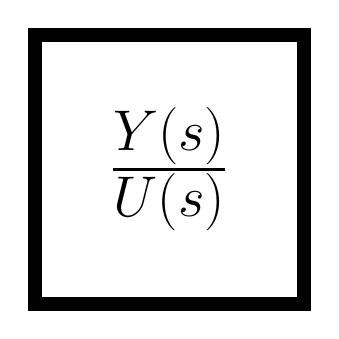
\begin{tikzpicture}
	\begin{axis}[domain=-1:1, tick style={draw=none}, ticks=none, ymax=1.1, ymin=-1.1, xmax=1.1, xmin=-1.1, line width=5, width=5cm, height=5cm]
		\node[text width=3cm, align= center,] at (axis cs: 0.0,0.0) {\Huge $\frac{Y(s)}{U(s)}$};
	\end{axis}
\end{tikzpicture}

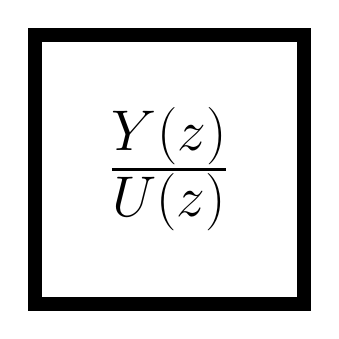
\begin{tikzpicture}
	\begin{axis}[domain=-1:1, tick style={draw=none}, ticks=none, ymax=1.1, ymin=-1.1, xmax=1.1, xmin=-1.1, line width=5, width=5cm, height=5cm]
		\node[text width=3cm, align= center,] at (axis cs: 0.0,0.0) {\Huge $\frac{Y(z)}{U(z)}$};
	\end{axis}
\end{tikzpicture}


\end{document}